\chapter{Experimental Setup}
\label{chp:experimental_setup} 

\section{Microphone selection}\label{sec:ch3_microphone_selection}

In our project, we use different kinds of experimental setups. 
The first setup is the Zoom H4n Handy Recorder. 
The recorder is able to record WAV files with a sampling frequency \( {F_{s}} \) of 96kHz and a quantization of 24 bit. We were also able to plug it directly into a computer, thus using it as the standard sound input device. 
However this limited the operating sampling frequency \( {F_{s}} \) to 48kHz.

To be able to record even higher frequencies, we use a Knowles Ultrasonic microphone connected to a National Instruments myDAQ device. 
The microphone should be able to detect frequencies up to 100kHz combined with the myDAQ that is able to sample with a \( {F_{s}} \) of 200kHz.

Since a lot of the information we are looking for is in a frequency range far above the hearing range of the human ear, we require a microphone that can capture these frequencies. 
The frequencies we are able to observe are limited to the Nyqyust frequency.

\begin{equation}\label{eq:ch3_nyquist_frequency}
F_{nc} = \frac{F_{s}}{2}
\end{equation}

This means that we are able to study the frequency response up to frequencies of 48kHz using the setup.
In original research, it is claimed that there is information for fingerprinting in this frequency range, thus we should be able to observe the phenomenons.

\subsection{Zoom H4n Configuration}\label{sec:ch3_zoom_H4n_configuration}\todo{Redundant section?}

The Zoom H4n Handy Recorder is set to Sterio Mode.
Further, the sampling frequency is set to 96 kHz and the analog to digital converstion is set to the maximum which is 24 bit.
The recorder provides a 237 Hz low cut filter, which is enabled.
These low-frequency frequency responses are not providing information that is critical for looking at the fingerprints and \todo{citation paper; Look at explanation from the original paper} \todo{Low cut filter not working??? Cannot be observed in plots ...} 

Since we do not have a remote controll for the recorder, we have to manually click the record button to start and stop our recordings. 
This means that we are touching the recording device, thus impacting the samples when the contact is happening. 
This is not critical for our setup, as we are recording a time interval of several seconds; only the samples in the timeframe when we are activly starting and stopping the recording are affected by the physical contact. 
However this makes it harder for us to do multiple recordings with the recorder in the exact same place, as touching the device will inevitably cause some slight displacement.

\subsection{Knowles Ultrasonic SPU0410LR5H Configuration}\label{sec:ch3_knowles_configuration}

\begin{wrapfigure}{r}{0.5\textwidth}
    \vspace{-20pt}
    \centering
    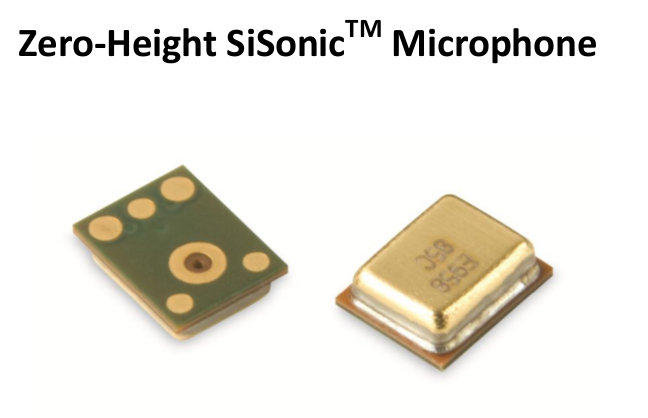
\includegraphics[scale=0.3]{knowles_microphone.png}
    \vspace{-20pt}
    \caption{Knowles Ultrasonic SPU0410LR5H~\cite{knowles_spec}}
    \vspace{-20pt}
    \label{fig:knowles_microphone}
\end{wrapfigure}

The Knowles Ultrasonic SPU0410LR5H microphone in \autoref{fig:knowles_microphone} is able to detect sound at least up to 80kHz with a -4dB sensitivity\cite{knowles_spec}.
To be able to record frequencies up to 100kHz, we need the National Instuments (NI) myDAQ~\cite{NI_myDAQ} to sample the sound at a sampling frequency \(F_{s}\) of 200kHz.
The microphone is connected to a 4.5V battery and directly in to Analog Input 0 on the myDAQ device. 

The myDAQ device has a built in an amplifier (OPA1642) seen in the hardware block diagram at page 4 in the myDAQ user guide~\cite{NI_myDAQ_userguide}. 
The OPA1642 has a gain of 60 dB at 10kHz and 40 dB at 100kHz seen in figure 5 at page 5 in the OPA1642 specification~\cite{TI_opa1642}.
With an input vaoltage of +-10mV, the nominal output is +-1V as illustrated in \autoref{fig:op_amp_illustration}
\todo{check this with Tim Cat Netland}

\begin{figure}[h]
  \begin{circuitikz} 
    \draw 
    (0,0) node[op amp] (opamp1) {}
    (opamp1.+) node[left ] {10mV @100kHz $v_+$}
    (opamp1.-) node[left ] {$v_-$}(1,0)
    (1,0) to[voltmeter, l=1<\volt>] (4,0);
  \end{circuitikz}
  \caption{Op Amp illustration}
  \label{fig:op_amp_illustration}
\end{figure}


\subsection{Brüel\&Kjær 4191 Configuration}\label{sec:ch3_bruel_kjaer_configuration}

Much like one of the lab setups~\ref{sec:lab_setup} from the original paper we use a Brüel\&Kjær 4191 microphone that is able to do precise measurements up to frequencies around 40kHz~\cite{bk4191_spec}.
The microphone is then connected to a preamplifier \todo{write about the preamp we used in the experiment} which is then connected to a Brüel\&Kjær 5935 microphone power supply and amplifier.
The output signal is then led into the NI myDAQ and further in to our computer, i.e. the adversary in this case.

\section{Processing and signal extraction}\label{sec:ch3_processing_signal_extraction}

The captured sound is stored in a WAV file.
This file is processed in our self written software, which utilizes libraries such as FFTW \todo{citation here} and libsndfile \todo{citation here}.
The samples are devided into windows \( W \), where \( \lvert W \rvert = 2^{n} \) where \( n \) is a non-zero positive integer.

The WAV file contains a sterio signal, but since our audio source is hardly a sterio source, we only need one of the channels for our furter processing. \todo{Reasoning about why we only need mono} 
In the WAV format, frames representing each sample is stored subsequently, such that the sample \( s_{f,c} \) represents the PCM \todo{Pulse-code modulation abbrevation} response for frame \( f \) channel \( c \). 
Since we have a stereo signal, we have that \( f \in \left [ 1, 2 \right ]  \), and thus the samples are ordered  \( s_{0,0}, s_{0,1}, s_{1,0}, s_{1,1}, ... , s_{n,0}, s_{n,1} \). 
To obtain a mono signal we simply ignore all frames where \( f \neq 0 \).

\section{Capturing audio fingerprint}\label{sec:ch3_capturing_audio_fingerprint}

Our guess, based on the original paper~\cite{original_paper}, is that the sound derives much likely from some coil whine around the CPU. 
Therefore we are positioning the microphones as close to the CPU as possible. 
When listening to the Lenovo T60p, we unmounted the keyboard letting us position the microphone on top of the cooling element for the CPU as illustrated in figure~\ref{fig:T60p_knowles_position}. 

\begin{wrapfigure}{r}{0.5\textwidth}
    \vspace{-20pt}
    \centering
    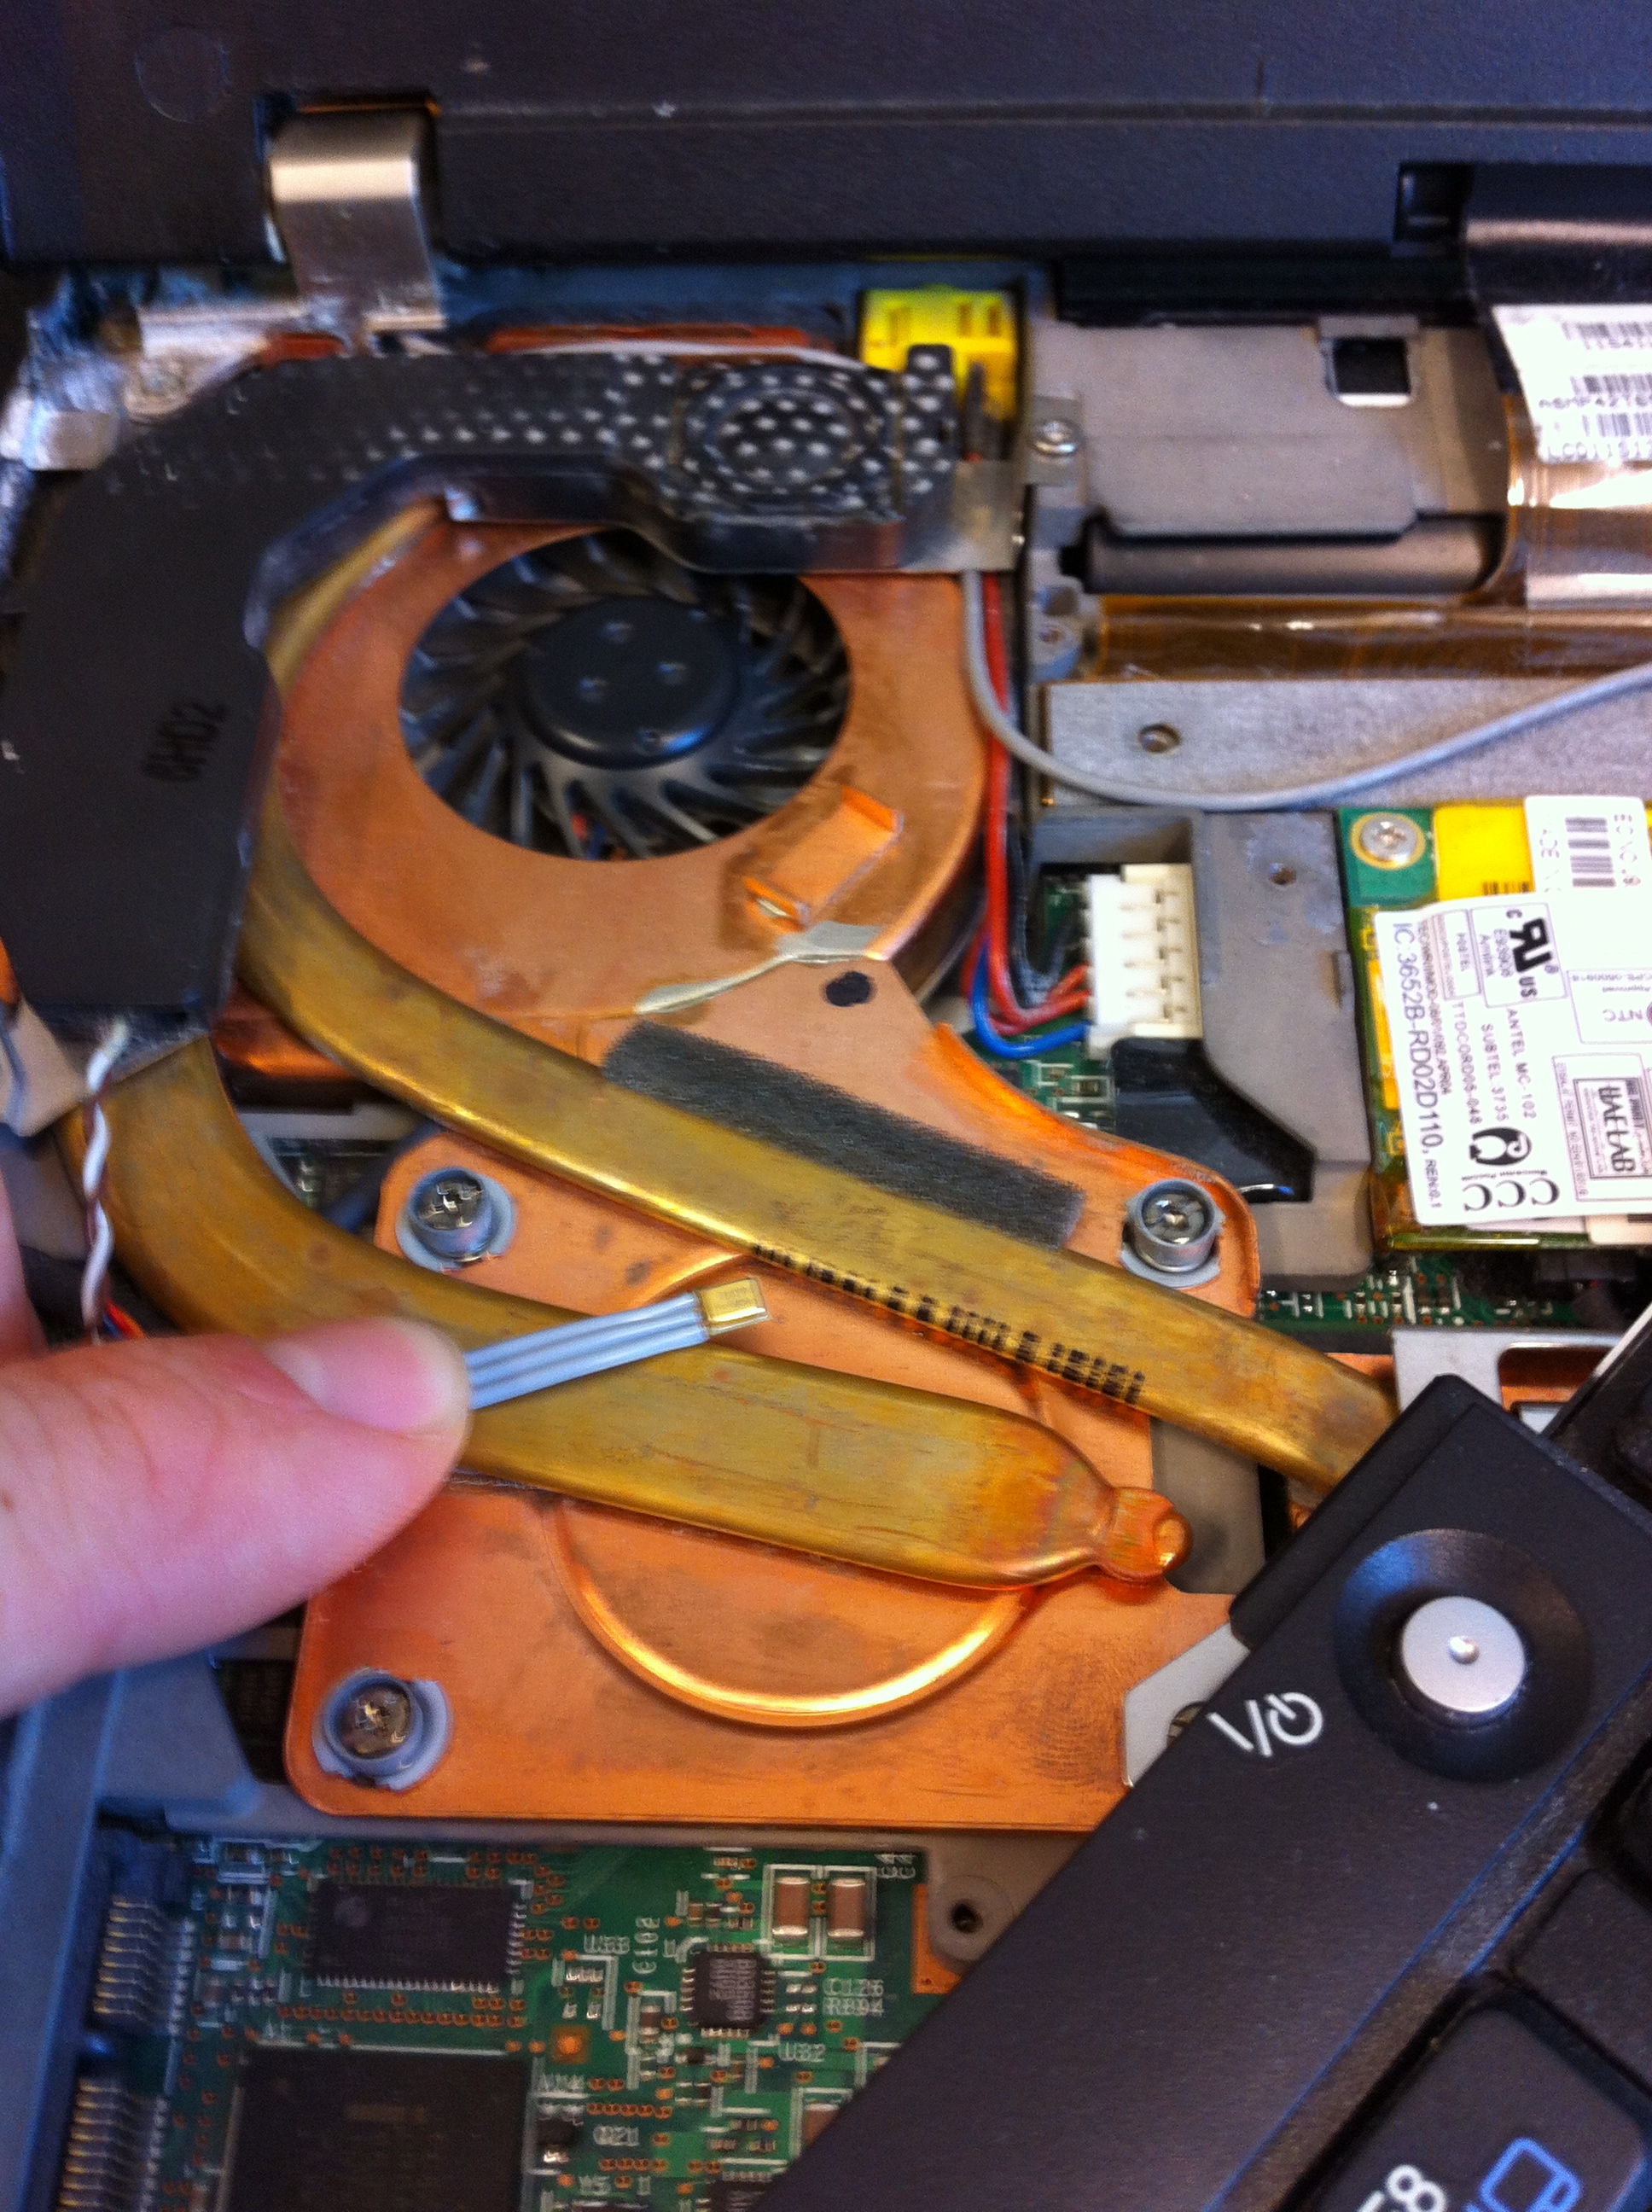
\includegraphics[width=2in]{T60p_knowles_position.JPG}
    \vspace{-20pt}
    \caption{The Knowles Ultrasonic SPU0410LR5H~\cite{knowles_spec} microphone position when recording close to the CPU on the Lenovo T60p.}
    \vspace{-20pt}
    \label{fig:T60p_knowles_position}
\end{wrapfigure}


\section{Experimental plan}\label{sec:ch3_experimental_plan}\todo{Put this in appendix}

Our experimental plan consists of different test cases on different subjects with different microphone setups. 
Each test case is performed with all microphone setups and with all test subjects. 

To calibrate each microphone, we are using a tweeter to play a sinus wave from a tone generator. 
The frequencies that will be generated are 10kHz, 20kHz, 30kHz and 40kHz.
After calibration, we will record the ambient noise where we are doing the experiment.
This is to eliminate other sources of noise when we are doing the experiments.
We will also do the experiments in an anechoic chamber, which will eliminate close to all other sound sources.

\subsection{Test cases}


\begin{enumerate}
  \item[CPU idle] Record when the CPU is idle. 
  We are doing this to find out what the CPU possibly might leak when doing nothing. 
  Then we perform a CPU load, micro instructions and finally decryptions.
  \item[CPU load] Exposing the CPU from low to high load.
  Read more about how we do the CPU load in chapter~\ref{chp:analyzing}.
  \item[Micro instructions] Read more about how we do the micro instructions in chapter~\ref{chp:analyzing}.
  \item[Decryption] As stated in the original paper, we should be able to detect when the CPU is doing a RSA decryption. 
  For this we decrypt an encrypted file with a RSA 4096-bit key using GnuPG v1.4.15~\cite{GnuPG_1.4.15}
\end{enumerate}

\subsection{Test subjects}
On all test subjects, we are planning to record as close as possible to the CPU. 
The following devices is tested:

\begin{itemize}[topsep=-1em,parsep=0em,itemsep=0em]
 \item Lenovo T60p
 \item Raspberry PI
 \item Dell Latitude D430
 \item Dell Latitude D400
\end{itemize}

\subsection{Microphones}
The microphones we use during our experments:

\begin{itemize}[topsep=-1em,parsep=0em,itemsep=0em]
 \item Knowles Ultrasonic SPU0410LR5H described in section~\ref{sec:ch3_knowles_configuration}
 \item Zoom H4n described in section~\ref{sec:ch3_zoom_H4n_configuration}
 \item Brüel\&Kjær 4191 described in section~\ref{sec:ch3_bruel_kjaer_configuration}
\end{itemize}